\chapter{Introduction}
%What is the purpose of this paper? What is the content of the next two sections?
Jeff Bay's "Object Calisthenics" \cite{bay2008} are nine rules that train the software developer to write better object oriented code.  He created concrete rules out of general software principals and patterns. These rules shall be applied in a short exercise, usually about two to four hours. With these concrete rules the trainee doing the exercise can improve his software development skills, which is helping him when applying general software principals and patterns to real world software projects. The exercise and the reasons for it are described in this chapter, in section \cite{i:exercising}.\\

%=== What shall be reached in the end of this paper?
This paper is divided into three chapters.\\

Chapter \ref{Description} describes Jeff Bay's rule and what let him establish the nine rules. It poses Jeff Bay's reasons for today's problems of software development.\\

The chapter describes every rule step by step. Within this description, a source code example is given. A bad example firstly exemplifies how the code looks like without the rule. A good example, validating the rule, then shows the advantages of the resulting source code when applying the rule. These examples are described shortly. After describing the examples, it researches concepts behind the rule. It describes the problems that would occur without the rule. After explaining the problems behind the rule and Jeff Bay's rule, a more detailed analysis ensues. In this detailed analysis, patterns and principals are described and ideas and concepts are examined. Section \ref{d:background} describes these principles detailed for every rule, step by step. In the end, the section \ref{d:discussion} furthermore discusses the rules shortly.\\

Chapter \ref{Evaluation} investigates possible tool support to validate the Object Calisthenics. First, the section \ref{e:advantages} describes general advantages of tool support. The section \ref{e:evaluation} goes through every rule presents the possibilities to validate the given rule. Advantages and disadvantages of the implementation are explained and a short conclusion of every rule is drawn. Section \ref{e:result} then summarizes the results of the evaluation of rule validation. Lastly, section \ref{e:future} further ideas of rule validation and links for further work.\\

The last chapter \ref{Prototype} describes a prototypical implementation done during this research. The prototype shows the practicability of the evaluation results.

\section{Exercising Better Object Oriented Programming Skills: a Concept by Jeff Bay}
\label{i:exercising}
Jeff Bay's "Object Calisthenics" \cite{bay2008} are an exercise to improve the quality of Object Oriented code. According to him, the chapter "will give new programmers an opportunity to learn best practices while writing their own code." \cite[p. 70]{bay2008}.\\

The book "The thoughtworks anthology. Essays on Software Technology and Innovation"\cite[p. 70-79]{oc2008} was released in 2008. The whole paper consists of thirteen chapters discussing various topics and ideas on how to improve software development. The essays discuses problems and ideas on languages, tool support, software principals and software quality. One of the paper's chapter describes the rules of the Object Calisthenics. Furthermore it shortly describes their purpose and outcome and why the author Jeff Bay created these rules.\\

All essays in the book \cite{oc2008} are written by developers working at the company "Thoughtworks inc". The company is well known for creating, designing and supporting high quality software. The company is to be said to be one of the most future oriented company in terms of technology and software principals. They describe themselves as "[\dots] a software company and community of passionate individuals whose purpose is to revolutionize software design, creation and delivery, while advocating for positive social change [\dots]" \cite{twWeb}.\\

%=== What are the Object Calisthenics in general (nine rules...) 
The Object Calisthenics are nine programming rules helping to write good object oriented code. But moreover the Object Calisthenics are an exercise to improve the quality of Object Oriented code. Good Object Oriented Code is hard to learn when coming from procedural code. Many developers think in Object Oriented code – but do they really write good Object Oriented Software? That is the question that Jeff Bay poses in his essay.\\

Usually the developer doesn't use these rules in real world project but applies them in short two hour exercises in which he designs and implements minimalist software with little requirements. This could be a Minesweeper or a Tic Tac Toe game for example. These training challenges should lead the developer to write better code and be more aware of code quality in real world projects.\\

With these little training sessions, the Object Calisthenics help to create highly object oriented code  in small projects. When applying the rules, the developers automatically fulfill many important software patterns and principals leading to higher code quality than the code would have without the given rules. By training developers to focus the rules they automatically apply various helpful and important software principals and software patterns. \\

The developer is supposed to "spend 20 hours and 1,000 lines writing code that conforms 100 "\%"  to these rules" \cite[p. 80]{oc2008}. He is convinced the developer will "break old habits" \cite[p. 80]{oc2008}. Furthermore he promises that the exercise will change the way "that you may have lived with for your whole programming life."\cite[p. 80]{oc2008}. According to Bay, this change is the result of the developer's need to rethink and lateral thinking. He is genuine that by this process the developers perspective on existing code and the way he will write code in the future will change radically. As just described this rethinking is only possible in small, lucid projects. This is for example a project with 1,000 lines of code, as suggested by Jeff Bay. \\

However, Jeff Bay's idea is that by this process of rethinking the code quality of the code written by the developer will improve.
Of course this will only work if the developer recognizes the ideas and principals behind the rules, and hereby accepts the positive outcome of the resulting code. Hopefully he is able accept the positive value of the resulting code. When he is working in real world projects he hopefully remembers parts of the rules, resulting ideas or principals and concepts behind the rules. Because of the improvement of his software development skill, he is then able to apply the concepts to real world project. The result is a tremendously improved code quality in the real world project.\\

Improving the quality of software's implementation by little training sessions - that is his idea, basically. Jeff Bay included also this idea in the name of the rules. The word "Calisthenics" indistinguishable describes the approach, the idea and the outcome of the exercise.\\

As already said, the background of every rule is described in chapter \ref{Description}.

%TODO checken: ist klargestellt, das (research seite 7):  - strict coding standards, used without doubts during the excercise ==> unerstand 100 percent pure object orientaiton "in perfection" in a small project. --=> Remember the lessons learned when coding  in the "wildlife". 

\section{Tool Support to Validate the Object Calisthenics}
%=== Describe the outcome of a tool validating the rules of the Object Calisthenics.
%=== How might it support the developer?

%=== How might the tool boost the speed and efficiency of the developer while doing the exercise?

%=== Say: Tool support is examined and elucidated in chapter 3.

%=== Say: Prototype in the last chapter: 4. 
The purpose of the Object Calisthenics was already described. However, in this paper the focus lies on the evaluation and prototypical implementation of tool support, validating the rules of the Object Calisthenics. \\

Evaluating the possibility to create tool support validating the Object Calisthenics is the main part of this report. It has two main advantages - efficiency and quality.\\

Providing tool support for the rules of the Object Calisthenics could improve the time the developer uses to conducts the exercise. This efficiency increase simply makes it easier to do the exercise.\\

Furthermore it might reveal rule violations that where not detected by the developer yet. Therefore it could guarantee that the developer sticks to the rules. This is a quality improvement. \\

Therefore, the next chapter  \ref{Description} describes the rules Object Calisthenics to understand the software principals and quality metrics behind the Object Calisthenics. 

As already mentioned, the ensuing chapter \ref{Evaluation} discusses tool support for every rule.  the prototypical implementation is described in chapter \ref{Prototype}.

\chapter{Object Calisthenics by Jeff Bay - Patterns and Principals}
\label{Description}
This chapter describes the patterns and principals behind the Object Calisthenics. 

Firstly, in section \ref{d:problemsprocedural} the advantages of the Object Calisthenics are described. Before explaining the advantages of Object Orientation, the problems of non object oriented code are discussed. 

In the second section \ref{d:background}, Jeff Bay's rules for better object oriented programming are described step by step. Every rule is described, explained and a good and bad example are given. The examples conduce to understand the problem and the solution given by the rule. Furthermore patterns and principals behind the rules are explained. 

\section{Problems of procedural code}
\label{d:problemsprocedural}
There seem to be problems with procedural, non object oriented code in software. By saying non object oriented software, procedural code is meant. Jeff Bay lists the most important ones in \cite[p.70]{oc2008}. These disadvantages and problems of procedural source code are explained in the following. 

\subsection{Problems of procedural code} 
In procedural code the behavior is described by step by step operations resulting in an algorithm. 

\subsection*{No bundle of data and behavior}
The operations, also called commands, in procedural code usually access multiple data structures storing and managing data during the execution time. In procedural code steps can be consolidated by using methods with output and input parameters. Methods can summarize multiple commands to an abstract step that can be executed by a caller. Therefore procedural code provides a solution for structuring algorithms.\\

But there is another problem remaining. By simply looking at the data structures, the developer cannot see possible operations on the data structure. Of course, he is able to see what is stored in the data structure. However, he is not able to see which operations can be executed on the data structure and how the data structure is supposed to be used. He can only get that information by reading through the algorithm step by step and remembering the possible operations on the data structure. In procedural code there is not clear coherence between the data structure and its problem specific operations. There is no solution for the problem of bundling data and behavior given in procedural software development. \\

Furthermore there is no encapsulation of the data structures, hiding the implementation from the abstract definition of possible operations. Also, procedural software lacks of encapsulation. The concept of scoping therefore realizing encapsulation is not given in procedural code. 

\subsection*{Maintainability}
\label{problem:maintainability}
The just described problem of the low cohesion of data structure and problem specific operations makes maintainability of procedural code hard. Source code of long lasting software has to be maintained years after the initial design and the first implementation. In old and large code bases changes are hard to conduct. This is because the cohesion of behavior and data structures and the bad encapsulation between the different data structures is low. To be able to compensate the cohesion, relatively much documentation and much time to read the code is necessary. Therefore the low cohesion makes the conduction of maintenance software changes hard. 

\subsection*{Not understandable}
Another problem, closely related to the problem of maintainbility, is the understandability of code. As already said, the problem of the low cohesion makes it hard to dedicate the operations to the data structures. The difficulty to dedicate operations to the appropriate data structures makes the understanding of the code hard. By  reading through a part of an algorithm, the developer does not know which operations will be executed on which data structure. Secondly, when there are multiple operations on many different data structures, the developer has to remember all these state changes of the data structures. Therefore procedural code is often hard to understand. 

\subsection*{No modularity}
\label{problem:nomodularity}
%cohesion shcon einfuerne, damit  in advantages of oo zur verfuegung steht
In modern software development the separation in different modules is a core concept.\\

Modular programming "breaks down program functions into modules, each of which accomplishes one function and contains all the source code and variables needed to accomplish that function."\cite{about}. In \cite{about} Juergen Haas also states that the concept of modularity enables the programmer to debug and maintain difficult source code more easily. \\

A module only contains all necessary information and operations to perform the steps necessary. All other information is not visible by the module, it is hidden in other modules that are responsible for other tasks. However, within one module the developer is not distracted by other operations or data structures that are not related to the module, because they are hidden. 

\subsection*{Structure}
As already said, procedural code is only structured in different algorithm steps. The data structures are can't be encapsulated. This makes structuring procedural code extremely hard, because there is no mechanism enabling the developer to give structure by hiding information. The only way to give structure is to sort different methods in different files. But even if a data structure and its functions are put in a different file, the data structure is not hidden from the other files. The data structure can be manipulated in every other position of the program.

\subsection*{Overview}
This point is closely related to the just explained problem of structuring the program. The only way to sort or separate something can be done by using separate files. But still, this does not solve the problem of information hiding and therefore an overview is not given.

In procedural code it is not possible to put problem related data into a abstract data types.

\subsection*{No reusability}
In procedural code it is hard to reuse code. This is a result of the missing encapsulation and the missing modularity that was explained previously.\\

As already said in procedural code, a method often interacts with many variables of the system that are not encapsulated. A method can interact with all system variables. This leads the developer to not separate the program into different parts with their own responsibility and their own well encapsulated data structures and operations. \\

When using multiple files in procedural code, at some point the order of inclusion of these files has to be determined. When another file is imported there is no guarantee that the included files does already execute an operation. Furthermore, cyclic dependencies can occur that have to be resolved manually. \\

However in object oriented software the concept of encapsulation, respectively scoping, of data structures is integrated in the concept of object orientation.  In good object oriented software every module and object has a clear scope and is well encapsulated. This makes it easy to reuse the object or module. Firstly, it's dependencies are clear visible. They are not order specific, because they do not determine the order of the inclusion of files, but they determine the types that are used by the class. Secondly, the inner state expressed by data structures is hidden from everything that is not part of the module. The developer does not have to apprehend other modules to change internal states of the module. Thirdly, the operations that can be executed on the object are well defined. The developer can document those interfaces to help developers using the interface to understand how the module or object works.

\section{Advantages of object orientation}
%TODO Ueberschrift zeigt Anfang princip oo saves us!
The described problems and disadvantages that where described in the previous chapter \ref{d:problemsprocedural}, led to the use of object orientation. 
%TODO describe history of ooo shortly. 
All in all it is generally stated that object orientation and its related principals saves us from the problems, described in \ref{d:problemsprocedural} and provides a proper solution. \\

According to Jeff Bay the change from programming in an procedural way towards programming object oriented style is hard to learn. "Transitioning from procedural development to object-oriented design requires a major shift in thinking that is more difficult than it seems" \cite[p. 70]{bay2008}. 
%TODO 2 te quelle die zeigt, dass das lernen von oo von procedural schwer ist
According to Jeff Bay, however, the procedural way of thinking is still in the mind of many developers. "Transitioning from procedural development to object-oriented design requires a major shift in thinking that is more difficult than it seems" \cite[p. 70]{bay2008}. %TODO hier 2 te qeulle und noch eien satz? sosnt halber absatz zitiert...
"Many developers assume they’re doing a good job with OO design, when in reality they’re unconsciously
stuck in procedural habits that are hard to break" \cite[p.70]{bay2008}.
Not only the problem of the difficulty to learn a different way of thinking and coding when changing from procedural to object oriented code is a problem. But also the fact that it is easy for a developer to write procedural code. The disadvantages of procedural code are do not occur immediately. Many of the problems when dealing with procedural source code occur late. That means that the developer does not get an immediate feedback about the quality of his code while writing it, but realizes the bad design of the procedural written code after he conducted a change. \\
%todo dies noch belege. Ist es nur die motivation oder steckt da ncoh mehr dahinter? was sagen andere?
%vielleicht in mf's refactoring
And even worse, when he is not realize the disadvantages of procedural code, 'there is no motivation for him to change that behaviour'. Furthermore when creating code and not maintaining legacy code it is generally easier to write procedural code than to write object oriented code. Creating procedural code is significantly easier than creating object oriented code in the first place. The creation and the management of objects and a good implementation of encapsulation is difficult. But the quality of these two features, that are special for good object oriented software, are hard to realize. Whereas implementing the same functionality in procedural code is significantly easier.

Therefore it is easier for the developer to write procedural code, than it is to write object oriented code. \\

Using the concept of object orientation helps to create software that as multiple advantages. These advantages are described later in this section. Before I will explain the advantages or core concept stated by Jeff Bay, I will summarize the characteristics and compare procedural and object oriented code very shortly. \\

Procedural code is more like a step-by-step description of sequenced commands. 	Seldom information hiding is used in procedural code. Furthermore multiple operations manipulate data, but there is no bundling of data and behaviour in one secluded unit. \\

In object oriented software however such a bundling in units exits. Data and behavior are put together in classes and packages. A unit using another unit uses the interface of the unit to determine possible operations, and uses it as required. The actual implementation and the actual data structures are hidden from the calling unit.\\
 
In object oriented software tasks that do not have the same area of responsibility, are separated. If a unit has to offer functionality where it does not the domain knowledge to implement it, it delegates the task to another unit, implementing the desired behavior. Otherwise the unit would not do exactly and only what it is supposed to do. To satisfy the definition of a module it need to have a high cohesion and should only do the one thing that is dedicated to that unit. The definition cohesion was already explained in \ref{problem:nomodularity}. Therefore the object delegates its work to other units that are dedicated to that well defined and specific task. \\
%TODO schlecht ausgedrucket
There is a third point that is typical for object orientation. The things that are represented in software not only mapped by representing a list of commands, but having concrete representations for the real world. These concrete representations are object that model real world things directly and bundle the behavior and representation of a real world object directly. 
This enables to separate in different models and make the models reusable. By doing so the particular modules are reusable and are simple and easy to use. 
This led object orientation to the four pillars of object orientation: encapsulation, abstraction, inheritance, polymorphism. These pillars are the generally accepted basic advantages of object orientation. \\

Jeff Bay however enhances the advantages by "core concepts" and "core qualities" that mark good object oriented code. The qualities are: cohesion, loose coupling, zero duplication, encapsulation, testability, readability and focus.
%cohesion, loose coupling, zero duplication, encapsulation, testability, readability and focus
Bay does not further explain these qualities. In the next paragraph I will go through all the qualities and explain them shortly. \\

Because Jeff Bay's exercise was already described in \ref{i:exercising}, after the description of the code qualities, the detailed explanation of Jeff Bays nine rules will follow. 

\subsection{Cohesion}
\label{cohesion}
Cohesion describes "degree to which the elements of a module belong together"\cite{cohesionBook}. It is a software measurement describing how strongly related pieces of functionality are. Therefore it describes how well the units of a system are grouped. When units, dedicated to a simliar purpose, are part of the same group and no nonrelated unit is part of the group, the group has a high cohesion. A module with high cohesion has strongly related and very focused responsibilities\cite{wiki:cohesion}. Generally cohesion is not described as an enumerable number, but one is distinguishing between high cohesion and low cohesion. Low cohesion is considered bad whereas high cohesion is considered good.\\

There are different advantages of high cohesion. In object orientation for example, when methods of a class have a similar responsibilities, the object tends to have a high cohesion. All object's methods are dedicated to the one task dedicated for the object. The object does not provide any other methods and does not perform any other tasks that are not related its actual task. Therefore it is easy for the developer to understand the behaviour of the object and to understand what the object is doing, when it is interacting within application. High cohesion can also enhance the readability of code, because the reader is not distracted by method calls that are related to other tasks than the dedicated one. It is ensured that the operations of the implemented methods is only related to the task that the methods shall perform. \\

Low cohesion in contrast is bad, because the just described advantages of focus, readability and easiness to understand. The cohsion is decreased from high cohesion to low cohesion, when different aspects are implemented in one class. The result is a system that is mroe difficult to maintain and to understand system. 

\subsection{coupling}
\label{coupling}
%TODO use "class A, class B"
Coupling is a metric that describes the knowledge of a class about its surrounding objects. Loose coupling can be described by two attributes. Firstly, if a class knows less about the surrounding classes and only uses well defined, generic interfaces to those classes. It does not have knowledge about the concrete implementation of the class. Secondly, if the state of a class does not depend on the state of another state, or at least only depends on the state provided by the class directly, and not by other classes provided by that class but only uses the provided methods. 
When this is not the case, the classes are strongly coupled. The "lack of coupling means that the elements of our system are better isolated from each other and from change" \cite{wiki:loosecoupling}. 
% TODO quote is wrong!
Because the changes of an classes interface, for example when conducting a refactoring, do only spread to the directly related neighbor classes, loose coupling is considered a good object oriented style. It is easier to change loosely coupled classes than strongly coupled classes. 
Another aspect of loose coupling is the \acf{DIP}. 
Martin describes the \acf{DIP} in \cite{cc} as following: "In essence, the DIP says that our classes should depend upon abstractions, not on concrete details" \cite{cc}.

\subsection{duplication}
If there is no duplicated code in software, then the quality of zero duplication is fulfilled. If there is no duplication of components or algorithms, the components are reusable and do not have to be rewritten in a similar way. In some cases the component can be slightly adapted, but in the end it is working for all parts of the software that use the component. 
The metric indicating no duplication in source code is called code duplication. 

\subsection{encapsulation}
When a class or a module hides its internal state it is considered encapsulated. When class B is well encapsulated and there are well defined methods that can be executed, then a class A using class B, can depend on the methods, therefore the provided operations. 
There is no part in the implementation of class A where it depends on a variable of class B. Then class A does not depend on the inner state of class B. Therefore class B can implement its algorithms and state management independent form all using classes. 
Well encapsulated classes "restict component's access"\cite[Encapsulation]{wiki}. Furthermore, well encapsulated classes "bundle [...] methods that implement operations on data"\cite[Encapuslation]{wiki}. The date is then "hidden behind the specified methods"\cite[Encapsulation]{wiki}.

\subsection{testability}
Testability described how testable a class or module is testable. There is no metric describing the degree of testability but there are some metrics describing the tests itself. 
On metric is code coverage. It is and indicator on how many lines of code are covered by tests. The line is regarded as "tested" when there is a test that is running through a line of code. It is not guaranteed that every line occuring in the code coverage metric is actually testing the related behavior of the line. 
The just described type of codde coverage is called "line coverage", because it counts the lines that are tested in a test run. There are also other types of coverages. These are function coverage, that indicate how many functions in the software are covered by tests. There is condition coverage %TODOD
And there is branch coverage, indicating how many of the possible branches of the program are covered by tests. 

\subsection{readablitiy}
% TODO hier stehen geblieben
Readability basically consists of three different aspects. 
The first aspect refers to the easiness of understanding a certain amount of source code. It is basically the metric for the quality readability.  The more source code can be understood within a specified amount of time, the more readable the code is. This makes readable code important. But it is one central qualities in software, because much time is spent with reading existing code. In \cite{cc}, Martin describes quotes Grady Booch and Dave Thomas on statements about the readability of source code. Grady Booch describes readability in the following way. "Clean code is simple and direct. Clean code reads like well-written prose. Clean code never obscures the designer’s intent but rather is full of crisp abstractions and straightforward lines of control." \cite[p. 8]{cc}. He clearly sets the focus the style of the resulting code. According to thim, the code should be very easy to understand and read like an easily understandable book. Dave Thomas focues more on the fact that readable code is also readable for others. Even more he the problem of naming variables, functions and units. Furthermore he states that minimal and clear dependencies make code cleaner and more readable, because it thereby is readily comprehensable. "Clean code can be read, and enhanced by a developer other than its original author. [..] It has meaningful names. It  Provides one way rather than many ways for doing one thing. It has minimal dependencies, which are explicitly defined, and provides a clear and minimal  API."\cite[p. 9]{cc}. \\

Two other aspects are important when looking at the readability of source code. It is generally known that well placed documentation at parts of the code that are hard to understand, help the reader to grasp the code he reads. Therefore good documentation enhances the readability of source code.\\

In \cite{cc} Martin describes the third important factor for ensuring readability. Martins "step down rule" is a rule ensuring the separation of different layers of abstraction. Classes or components describe different levels of abstractions. Abstract level classas are usually the "top-level" entry point when calling a module or a libray, whereas low level classes execute very problem specific operations. The step down rule states that this hierarchical ordering of functions exists. In addition it says that all functions that are declared in one class should all be on the same level of abstractions. Furthermore very method of a higher level should only call functions declarated on a lower level. The result is a composition of functions going from a abstract to a concrete level. For the reader of the code it is easier to understand the resulting code because he know exactly in which level of abstraction he is located. He can therefore navigate more easily to the desired code positions. Furthermore he doesn't have to understand every detail of the whole code, but can use the the higher levels of abstraction to understand quickly what the code is doing. 

\subsection{focus}
\label{focus}
The last quality Jeff Bay describes in \cite{oc2008} is focus. Focus is the description of "doing one thing". Every unit is dedicated to one task it has to manage and fullfill successfully. Focus describes not only this dedication, but furthermore states that the unit shouldn't do anything more. Consequently, the module contains no operations that are not related to that task. If it has to trigger other tasks that are not related to its dedication, it uses methods on other units that are specialized on this task. This means the module delegates all tasks that are not part of its dedication to other units. These units themselves are dedicated to the delegated task. Focus is very similar to the just described quality coupling in chapter \ref{i:exercising}.

------------------------
% TODO hier stehe geblieben

\section{The Rules and their Background}
\label{d:background}
 The instruction on how to conduct the excercise was already describe in the beginning, in chapter \ref{i:exercising}. This chapter describes the rules of the Objct Calisthenics itself. \\
 In the chapter I will go through every rule, step-by-step. Every every section will describe the patterns an principals behind the rules, elucidate design patterns and best practices that correspond with the rules. Each rule will furthermore exempify the rule by a good and a bad example. 

=== FOR EACH rule/subsection IN rules/subsections: 
Every rule is described one after the other with the information that is already documented in the commited work of the "research" phase: 

 - Explain the rule. Use quotes of paper. 
 
 - Every chapter gives short explanation, a good and a bad example. These examples are explained shortly. 
 
 -  Furthermore every chapter describes the software patterns and software principals behind every rule. These are for example design patterns, software principals and best practices. 
 
 - Refer to other sources to be able to explain clearly but shortly. Summarize complex patterns instead of explaining every pattern and principal in detail. 
 
 - Make sure the principals behind are easy to read: A advanced reader should not be bored by detailed explanation and a beginner reader should be able to understand the main message and idea behind the principal and idea.
 
 - The outcome of every rule is then summarized.

\subsection{Rule 1: "Use One Level of Indentation per Method"}
\label{describe:rule1}
With his first rule, "Use One Level of Indentation per Method", Jeff Bay's tries to tackle the problem of low cohesion and ensure that one class is only operating on one level of abstraction. These two problems and their solutions are presented in the following. 

The metric cohesion, which was already described in \ref{cohesion}, describes how well an object is focused and how well it is dedicated to one single task. The principle of "doing one thing", that Fowler describes in \cite{cc}, was already mentioned in \ref{focus}. Jeff Bay's Rule "Use One Leve of Indentation per Method" takes the principle of cohesion which is often applied on a class level and applies it on the method level. By doing so he ensures that a method is only doing what it is supposed to do and therefore delegates all non-relevant tasks. \\

There are two important principles behind the rule. 

The idea of delgating all non releveant work and therefore raise the cohesion can be done in the following way.
This is ensuring that the method is only manipulating data that is related directly to the method. This means ensuring the method does not mainpulate data that is accessed via muliple getter methods, other method calls or iterations. Such an access would change data that is not related direclty to the object itself. Therefor a foreign object would mainpulate the data of another object - instead of calling a method on the object. As already described other, just called "forign objects", can be accessed via method calls and control structures like while, for and do-while loops. Therefore when accessing an object with nested control structures, the methods is likely to change such "foreign object". There are two rule by Jeff Bay that prohibit such a "deep" access to those "foreign objects"' data structures. One is this rule, restricting the nesting of control-structures and the other rule is Rule 4 "Use only one dot per line" restricting the "deep" access via chained method calls. \\

As already mentioned, there is another principle that plays an important role, when looking at the rule. The idea of "one level of abstraction", which is described by Martin Fowler in \cite{cc}, is the other one. The basic ide of the "one level of abstraction" principle was already introduced in \ref{readability}. Martin Fowler states that a method should only operate within one level of abstraction and delegate all other tasks that are on a lower level to another class. Fowler states the rule as important, because it hard for humans to follow. "This may be the hardest of these heuristics to interpret and follow. Though the idea is plain enough, humans are just far too good at seamlessly mixing levels of abstraction". When a method is operation on two levels of abstraction, no always, but often using nested control structures in order to acces the "deeper" objects and to conduct data manipulation on a lower level. Transfering those operations no only results in a better abstraction. After a split up of tasks in oebject on different levels, the cohesion of the objects raises. Furthermore the object on a abstract level does not have to do operations on a low level, but is using another object to undertake the task. The result in many cases is that the object on the abstract level does not have to use that much control structures do perform the task, because it simply delegates all work that is not on its abstraction level. Therefore the nesting of control structures disappears automatically. In his Rule, however, Jeff Bay prohibits the nesting of control structure and therewith forces the developer to use differen levels of abstraction ab initio. \\

The following code example describes a bad and a good example of the rule. The first example is showing a possible implementation and the second example is showing a refactore example, which satisfies the rule and as a high cohesion and only operates on one level of abstraction. 

For reasons of simplicity, the following java examples do not contain imports and the main method is always in the class that is used first. 
\\
The problem implemented to exemplify is quite simple: A school has multiple classes with students. The goal is to get the avearge age of all students in the school. 

\lstinputlisting{listings/rule1/example1/School.java}
\label{listing:rule1example1}

As the listing \ref{listing:rule1example1} shows, the method \textit{count} simply iterates over all classes of the school, then reads out all students of the class and counts their number. This operation uses nested for loops to determine the number of students. A first improvement would be to use multimple methods to get rid of the nested control structures. This is depicted in \ref{listing:rule1example2}. In this example, the control structures are not nested anymore, but method calls are used to conduct the counting of the deeper data. The deeper data in this case are the \textit{Student}s because their are contained by the \textit{SchoolClass}. 

\lstinputlisting{listings/rule1/example2/School.java}
\label{listing:rule1example2}

Even if \ref{listing:rule1example2} now fullfils the rule, there is still problem remaining. The class \textit{School} is still operating on the data that is contained by the class \textit{SchoolClass}. However the number of students in a school and the number of students in a class are two different concerns and they should not only be separated but be well placed in their corresponding classes. Then the the result is a higher cohesion, because the operations are placed perecisely at the classes. Therefore extracting the method that is counting the students of a class to the \textit{SchoolClass} is a step, improving the code even more. Listing \ref{listing:rule1example2:school} and \ref{listing:rule1example2:schoolclass} show the two classes with their corresponding counting methods, that are now located to the proper classes. 

\lstinputlisting{listings/rule1/example3/School.java}
\label{listing:rule1example3:school}
\lstinputlisting{listings/rule1/example3/SchoolClass.java}
\label{listing:rule1example3:schoolclass}
\\

The example shows exemplifies how Rule 1 "Use One Level of Indentation per Method" can improve the readability of code and the cohesion of the classes. The resulting classes are therefore easier to test, easier to understand and more focused on doing on dedicated task. The graphic in \ref{picture:rule1abstraction} shows exactly this. The operations on a deep abstraction level or operations on nested structures are not done on the abstract level. In contrast, the abstract level uses the lower level object to conduct low level operations. 

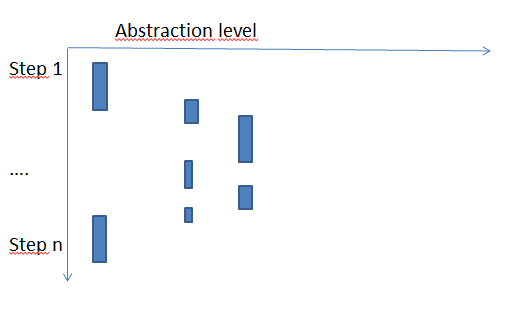
\includegraphics{Bilder/Rule1Abstraction.PNG}
\label{picture:rule1abstraction}

\subsection{Rule 2: "Don’t Use the else Keyword"}
\label{describe:rule2}
Jeff Bay's Rule 2 "Don’t Use the else Keyword", tackles the lack of understanding and usage of polymorphism. 
In \ref{oc2008} he states that many developers learn if/else constructs from day one. Therefore they are used to the usage of the construct. Even worse they learn the proper usage of polymorphism later on in their career. As a result the "way of thinking" in if/else constructs is still firmly established in developers' brains.
\\

As commonly stated, the exesive use of conditionals leads to code that is hardly readble. \cite{gof} also state that. "Like long procedures, large conditional statements are undesirable" \cite{gof}. Even worse, it leads to code duplication because the code with a lot of conditionals "is difficult to extend and to modify"\cite{gof}. This is because the deveoper does not see the usage of an if/else construct from the outside of the classe. Therefore if he does not know the class where object is used, he simply rewrites the behaviour that is already implemented in another method. Assumed there would be an object that had a clear description of the implemented behaviour and could be reused, then this erros would not occur. Furthermore the conditional within the method could also be implemented by different implementation behind a common interface, which is the basic idea of polymorphism. The setting of the direction would then not happen when passing the if/else construct, but the method would simply call another method of an object and the concrete implementation of a common interface determines the code that is executed. 
\\

In order to increase the reusability and conduct a better separation of concerns, Jeff bay restricts the usage of if else constructs, conretely the usage of the else keyword.
\\

There are several ways to reduce the usage of if/else conditionals and increase the overview and readability of the coding. The three ways of doing so are: early return, the Null Object Pattern and the Strategy or State pattern. These three approaches are exemplified in the next paragraph. 
\\

\subsection*{Early return}
Early return is a very simple way of decreasing the amount of if/else conditionals. Its goal is mainly based on removing unused else keywords. Listing \ref{listing:rule1example1} shows method with conditionals. The code also contains "else" keywords, even if they would not be necessary. When the block of the first if clause would use the return statement to early-return from the method, the else keyword would not be needed.
\lstinputlisting{listings/rule2/example1/}
\label{listing:rule1example1}
\lstinputlisting{listing/rule2/example2/}
\label{listing:rule1example2}
The second example, shown in \ref{listing:rule1example2}, shows the solution that was just proposed. As clearly visible there is no else keyword used anymore, but the control is also done by early returns. The advantage of this approach occurs when reading through the method stop by step. When seeing a return statement while reading through the method, the developer know immediately what happens. The reader of the method know that no other statement "weiter unten" of the method will be executed. It is very clear that the method "weitergeben " the control and that the execution is continued in the method of the callee. There is no long decision making by conditionals that navigate through the different cases anymore, but a clear end of the method - simliar to the semicolon or the dot in a sentence. Therefore, according to Jeff Bay, the practice of using early returns the readabliity is increased. \\

However others state that the opposite is the case and that the variable that is returned should always be defined at the beginning of the method. This makes use of the advantage that the developer already knows at the beginning of the method which variable is returned - a clear advantage in contrast to the early return approach. However, when reading through a method the developer always has to remember the variable that is returned and how it was changed. Furthermore, when returning a default value, the value is initialized in the beginning of the method - but the return statement and the return variabla are in the end of the method. Therefore the developer might have to look up the default value of the variable again. Whereas when using the the early return approach, this is prevented more likely. ???? genua genug???
\\

\subsection*{Null Object Pattern}
The use of the Null Object Pattern is way of getting rid of if/else constructs. The pattern is mainly used in static typed language, like Java for example. When a method is returning the value null, a problem occurs for the callee. He has to check with a condition if the reference on the return value is null or is null. An example for such a null check is shown in \ref{listing:nullobject1}. This constructs tries to achieve the execution of some lines of code only if a value is not null. However this has to be checked with an if condition. With the Null Object Pattern, polymorphism instead of if contisions is used to achieve the shown behavior.
\begin{lstlisting}
Object value = a.method();
if(value == null) {
	...
}
\end{lstlisting}
\label{listing:nullobject1}
The Null Object Pattern commonly has two implementation behind one common interface. One implementation however contains the code in which of the if clause's body that is shown in \ref{listing:nullobject1}, and the other object simply contains no code. The two classes are shown in the following. The \ref{listing:nullobject2} shows the Null Object itself and the other listing \ref{listing:nullobject3} shows the implementation containg the code. Within the method \textit{method()}, a concrete implementation of the common interface \ref{listing:nullobjectoperationinterface} is returned. If the object shall be \textit{null}, an implementation of the Null Object \textit{NullObject} is returned, if not the \ref{listing:nullobject3} is returned. By doing so, the call check of the conditions in the calle disappears, as depicted in listing \ref{nullobject4}.
\begin{lstlisting}
Object value = a.method();
if(value == null) {
	...
}
\end{lstlisting}
\label{listing:nullobject4}

The callee shown in \ref{listing:nullobject4} got rid of the if/else construct by the use of polymorphism. Another advantage is that the behavior of the object is not in the callee object, but is pushed within the object itself with the use of polymorphism. The result is a better allocation of the behavior to the objects.
\\

\subsection*{State and Strategy pattern}
The third way of getting rid of else keywords is via polymorphism - concretely the state pattern. A conditional structure has the one and only task to execute an additional block of statements or to decide which block is executed. In object orientation this can also be conducted with the use of polymorphism, and this offers multiple advantages, that will be explained later. 
The use of polymorphism means, in most cases, applying the strategy pattern. This will be explained firstly. \\

\\
The strategie pattern is a software pattern allowing different polymorphic implementations, that are hidden gehind a common interface. Which version of the method is executed is not determined within the object itself, but the concrete implementation of the object is determined by another object. The used implementation is "plugged" in by a deciding instance that determines the strategy that is used. The object itself, however does not care about the object that is used anymore, but simply calls the method of the common interface. The strategy pattern is used to create configurable algorithms with different behaviour of the implementation\cite[p. 349]{gof}. The output on a given input however is defined by the common strategy interface. The \acf{UML} diagram of the strategy pattern is shown picture \ref{picture:strategypattern}. An example of this is shown in listing ???. The first example shows a method not using polymoprhism, and the second, refactored example, shows the same method with polymorphism.

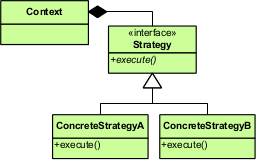
\includegraphics{Bilder/StrategyPattern}
\label{picture:strategypattern}

%% TODO codebeispiele einfuegen und kurz erlauter.
% TODO notzen kontrollieren - alles dabei?
%% TODO darstellung grafisch strategy pattern

%% TODO nur kurze erlaeuterung des state pattern
Like the strategy pattern, the state pattern is a behavioural software pattern as well. The state pattern can be seen as specialization of it. The state pattern also makes use of polymorphism. In contrast to the strategy pattern, the implementation used next can be changed by an implementation itself. In the state pattern, the different implementations of the common interface are representing the object's state. The objects state is expressed by the concrete state implementation, that is hidden gehind the common interface, which is valid for all states. Therefore a state can change the state to another state.\\

The \acf{UML} diagram of patter in shown in \ref{picture:statepattern}. The graphic shows the \textit{Context}, in which the \textit{State} is used. The \textit{ConcreteStateA} and the \textit{ConcreteStateB} are the concrete implementations of the common interface \textit{State}. The state implementations  \textit{ConcreteStateA} and \textit{ConcreteStateB} can change the state to another state. They can change the state to every implementation of the \textit{State} interface, therefore \textit{ConcreteStateA} can change the state to \textit{ConcreteStateB}.
All in all, the state pattern is clean way to encapsulate the change of behviour during runtime. In this patter not only the concrete implementation is encapsulated like in the strategy pattern, but also the transition from one state to another state is well encapsulated. \\
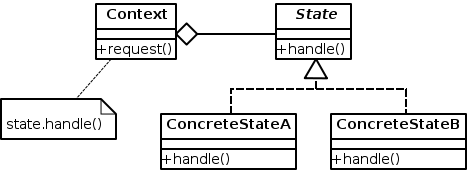
\includegraphics{Bilder/StatePattern.svg.png}
\label{picture:statepattern}

The just described strategy and state pattern make heavy use of polymorphism to bettern encapuslate code. They break procedural text lines into well encapsulated units\cite{gof}. The resulting code is easier to reuse and to modify and "makes them interchangeable"\cite{gof}. The interchangable polymorphic units should follow the \acf{LSP} rigorously.\\

The \acf{LSP} states that "a computer program, if S is a subtype of T, then objects of type T may be replaced with objects of type S (i.e., objects of type S may be substituted for objects of type T) without altering any of the desirable properties of that program (correctness, task performed, etc.)."\cite[Liskov Substitution Priniple]{wiki}. When a class overrides a method of a class or implements a method of an interface, the implementation should always behave as given by the abstract method definition. Therefore it is the principle that a subclass of a class (or an interface) should behave exactly as stated in the documentation of the abstract or overwritten method. In the result the output of a given method with a given input, is always the same and independant which of the polymorphic implementations were used. \\

 To guarantee the correctness of the class that is using the interchangable classes, each of the concrete implementations of those classes have to behave exactly as their abstract specifications eg. interfaces. There interfaces should be well documented and provide a clear description of what is expected to be the output on every possible given imput. The documentaiton can then describe the speicalties of the concrete implementations. However, under no circumstances the subclasses should disagree the interface's documentation but should follow the \acf{LSP} very strictly. \\

 All in all, these patterns enable the developer to "move multiconditinals and branches to own strategy [or state] classes"\cite{gof} and by this dramatically reduce the use of conditionals. By pushing login into interchangable own components, the cohesion of the class increases. It has less if/else conditionals and is, in result more readable and focused. The focus increases because the class does not determine the code to apply with conditionals to then treat them differently. Instead it uses method calls with the hidden and interchangable logic. To engage developers to use the described patterns and to benefit from their advantage, Jeff Bay permits the use of the \textit{else} keyword with this rule. 

\subsection{Rule 3: "Wrap All Primitives and Strings"}
Jeff Bays third rule "wrap all primitives and strings" tries to force the developer to push logic close the data. The basic problem this rule tackles is that most primitive values only relate to their meanding  by its varable names. \\

Primitive values however are variously used in software. They occur as parameters, loop counter, return values and temporary variables. However, in all of these cases the meaning of the variable is only reflected by its name. They reflect meaning, but at the same time do not offer the associated behavior. In the following, a bad and a good example is shown. \\

To explain this issue vivid, the following, bad example is given. The example used here is very simple. Imagine rolling a dice. The number, generated by the dice indicates the number of jumps you have to do. In the application the random method represents a complex process. The application however, consists of two classes. The \textit{Dice} represents the real world dice and is accountable for generating a random number. The other class, \textit{Game}, triggers the action of rolling the dice. Furthermore it is responsible for printing the results of the dice. The game represents how to process with the result of the data.   \\

The first example is depicted below in listing \ref{listing:rule3example1}. As you can see, the behaviour that indicates the number generated by the dice is indicated by the \textis{Dice}. However resulting number is returned by the dice. With this number, the \textit{Game} determines how the  display shall be displayed. The \textit{Game} takes uses a for loop iteration to process the data. The processing of data is represented by this loop. The fact that the resulting integer of the \textit{Dice#roll()} method is used to iterate is only represented by the variable name of the varible. Therefore if there are many different or more complex data pricessings, then it gets confusing very fast. How well code is understood is only represented by the variable names. From where the data is manipulated can only be determined by knowing the program or reading the documentation. This is because the behaviour is not located where the data is. This bad example shows this very clearly. The behavior that is determined by the \textit{Game} is only the way of printing: \textit{System.out.println()}. The other code, the for loop in this case that represents the complex processing of data, is not determined by the \textit{Game}. It is rather determined by the \textit{Dice}. 
\lstinputlisting{listings/rule3/example1/Game.java}
\lstinputlisting{listings/rule3/example1/Dice.java}
\label{listing:rule3example1}

The second example shows the first example, but re-written. In this example, the behavior is very close at the data. As you can see, the \textit{Game} now only determines the way of displaying the data. The processing is done by the \textit{Dice}. As a result, the \textit{Dice} now has handle the iteration and the text that is printed. By letting the dice determine this behavior, in this case the text that is printed and the iteration, only the \textit{Dice} know how to handle the generated results. All other classes that make use of the \textit{Dice}, can only manipulate how the result is printed via the \textit{Action} interface. 
When considering more complex code with multiple operations and data sets, this way of programming would not lead to confusing code. Because, in contrast to example one, the behavior that can be used to mainpulate the data is at the same place like the data. The behavior is not scattered in classes using the domain object \textit{Dice}. Furthermore the possible operations on the data can be only changed by changing the class that is providing the data. This makes the represented process of "rolling a dice" more transparent. If there is a extension for this process, then the change will be done in the \textit{Dice} class. Whereas in example one, the change could have been made anywhere. But then nobody else that used the \textit{Dice} would be informed about such a change, and therefore there is high risk of code douplication. 
\lstinputlisting{listings/rule3/example2/Game.java}
\lstinputlisting{listings/rule3/example2/Dice.java}
\lstinputlisting{listings/rule3/example2/Action.java}
\label{listing:rule3example1}

\\

The idea of pushing behavior very close to the data comes from the approach of \acf{DDD}. The idea of \acf{DDD} is to privide a domain model that represents problem specific scenarios. All problem specific behavior and all cases that represent the real world are represented by the domain model. The domain model if furthermore free of framework specific ???things??? like annotations or imports. The idea of \acf{DDD} comes from Eric Evans and he firstly presented it in \cite{ddd}. 
In \cite{ddd} the author separates between different types of objects. These are presented shortly in the following. 

\textbr{Entities} are the |top level" representations of the domain model. They provide the main entry point in the representing process. For example, this could be a class \textit{Contract} in a software that manages sales. 
A \textbf{Value Object} is an object containing attributes, but has no conceptual identity. This is the counterexample for an object that bundles behavior and data. 
An \textbf{Aggregate} is a collection of objects. Because the aggregate bundles multiple other objects, it is the object responsible for changes of its associated objects. It is the counterpart for all objects that want to conducte changes in the top level as well as in the sub objects. 
A \textbf{Service} offers operations that are not domain dependant
\begin{exampleblock}{Beispielblocktitel}
        Beispielblocktext
\end{exampleblock}





















%%%%%%%%%%%%%%%%%%%%% BAD exmaple, becaus eit does not show rule 1----Second, better example, -------

The following code example describes a bad and a good example of the rule. The first example is showing a possible implementation and the second example is showing a refactore example, which satisfies the rule and as a high cohesion and only operates on one level of abstraction. 

For reasons of simplicity, the following java examples do not contain imports and the main method is always in the class that is used first. 

%\lstinputlisting{listings/rule1/bad/HtmlHello.java}
\label{listing:rule1bad}

The example \ref{listing:rule1bad} shows a class used to create an \acf{HTML} element containing an auto incremented identifier \textit{id} and a String \textit{content}. In the method \textit{sayHello} an \acf{HTML} element is assembled an printed on the given \textit{PrintStream} of the method. The method appends the \acf{HTML}, a technical markup language and a domain dependent variable, and the\textit{content}, to the printer. The techincal \acf{HTML} is a formatting information on a low level. The content however is a domain dependent information, that is not dependent on the markup that is used. This is a violation of the "one level of abstraction" principle.\\

A solution is to extract the markup from the domain dependent information. In the following, an improved version of the problem is shown. In this example the high level information \textit{content} and the low level markup information are separated strictly. The new class \textit{HtmlElement} now represents a \acf{HTML} element with an \textit{id} and a \textit{content}. The class depicted in listing \label{listing:rule1good:element} is listed show the \textit{HtmlElement}. 

%\lstinputlisting{listings/rule1/good/HtmlElement.java}
\label{listing:rule1good:element}

Even if the new introduced class \textit{HtmlElement} is on a low level, very close to the markup language and not domain dependant, it is abstracting a simple structure of a regular \acf{HTML} element. Therefore the class can be reused by other classes 
%%%%%%%%%%%%%%%%%%%%% BAD exmaple, becaus eit does not show rule 1




asdf
\subsection{Rule 4: "Use Only One Dot per Line"}
asdf
\subsection{Rule 5: "Don't Abbreviate"}
asdf
\subsection{Rule 6: "Keep All Entities Small"}
asdf
\subsection{Rule 7: "Don’t Use Any Classes with More Than Two Instance Variables"}
asdf
\subsection{Rule 8: "Use First-Class Collections"}
asdf
\subsection{Rule 9: "Don’t Use Any Getters/Setters/Properties"}
asdf
\section{Discussing the Rules}
\label{d:discussion}
\ref{d:discussion}
=== This chapter is discussing the rules shortly. 

=== Use quotes from Jeff's text: He also gives a short summary of his text in the end

\subsection{Similarities}
=== Are there similarities in the rules? Is it possible to categorize the rules in terms of: 
 - Do they have the same intention?
 - Are they related to the same "big picture" idea (example: encapsulation or abstraction) 

Categorize rules: Are there similarities from perspective of principle? ??? Together with next chapter?

\subsection{Precedence}
=== Make clear that this is my own estimation and not related to Jeff's text. Prioritize the rules. 

=== To be determined: How long is this chapter?

\begin{itshape}
// Yada yada yada: 
Own estimation: what's the most important rule? 
What do I think?
What does the author think? 
Reason with descriptions and examples given
\end{itshape}

\subsection{Conclusion and Outcome}
=== Give a short and precise conclusion of the Object Calisthenic: Purpose, exercise, stuff to learn, skill improvement. 

=== Also Summarize what most of the rules are about: 

RESERACH page 21: 

- behaviour and operation oriented

- LoD and loose coupling

- talk to friends

- talk the protocol specified by the object's operation

- Next page: conclusion, no else ,naming, 

all in all: Duplication of code and idea
==> "Simple and elegant Abstractions"


\chapter{Tool Support to Validate the Object Calisthenics - Evaluation}
\label{Evaluation}
\section{Advantages of Tool Support}
\label{e:advantages}
=== What is a tool? Why do tools help? What makes tools strong? Why do tools matter for developers?
Possible outcome of tool support for the OC's? Already described in the Introduction (chapter 1). Describe this more in detail here if necessary. 
\section{Working Environment}
=== Describe AST generally. Say that Eclipse provides types representing the parts of code syntax. This is seen as given. 

=== Refer to other references explaining AST.

=== Describe shortly how it is possible to do an AST validation with eclpise. 

=== Say that: "Eclipse" terms for AST nodes are quite similar to general terms for java's nodes in ASTs. In this report the standard terms are used. These are not further described in this paper.

--> Example: Describe that "MethodDeclaration" consists of different other nodes representing the declaration of a method. Describe the structure of the child nodes of the node as far necessary. Do not embark on a discussion about what exactly is allowed as method declaration. 

=== Therefore: Give reference for questions about "parameter", "type", "class", "expression" or "statement".
Say that the validation in the next section is exactly implemented as described. One validation implementation example is explained exemplary in the Prototype chapter.

\section{Evaluation of Rule Validation}
\label{e:evaluation}
=== Say that the prioritization of the rules (in terms of the rule validation) and the "ranking" is given in the end. The sections of this chapter are "rule specific", even if the next subsections refer to each other.

=== FOREACH Rule/Subsection IN Rules/Subsections:

 - Similarities found out in description may be similar in this validation? Categorize the rules in groups to form a validation perspective. (E.g.: Validation of rule y is very similar to the validation of rule x that was already explained.)
  
 - Use examples given in description chapter to describe the typical structure of the rule. 
 
 - Explain "the positive case": What is the positive structure, satisfying the rule. Where does a rule violation occur when the structure is not fulfilled. (Example: Positive case: maximum of 2 instance variables. If not fulfilled: Discussion Rule violation information occurs on the level of the class or on the level of the third instance variable?
 
 - What checks have to be done for the validation?
 
 - Discussion of 'rule dependencies' within one rule (example: wrapper has to determine possible wrapper classes first before beeing able to indicate the use of a primitive/string in a non-wrapper class...)
 
  - --> solution found/no solution found
 
  - Therefore: Be self-critical: Now, were a "solution" is found (or not), describe the problems that occur with the described implementation
  
 - If there are cases where the rule cannot be validated: Why is it hard to validate. Where does the validation fail? How is it possible to "trick" a good implementation (Example: wrap of primitives can be "tricked" with 'return new Wrapper(instancevariable)'...) 

\subsection{Validation of Rule 1}
Cool, I can draw trees: 

\begin{tikzpicture}
[font=\small, edge from parent, 
    every node/.style={top color=white, bottom color=black!10, 
    rectangle,rounded corners, minimum size=6mm, draw=black!75,
    very thick, drop shadow, align=center},
    edge from parent/.style={draw=black!50,thick},
    level 1/.style={sibling distance=3cm},
    level 2/.style={sibling distance=1.2cm}, 
    level 3/.style={sibling distance=1cm}, 
    level distance=2cm,
    ]
    \node (A) {A} 
        child { node (B) {B}
            child { node {B1} 
            edge from parent node[left=.5em,draw=none] {$\chi^2$} }
            child { node {B2}}
            }
        child {node (C) {C}
            child { node {C1}
                child { node {C1a}}
            }
        child { node {C2}}
        child { node {C3}
            child { node {C3a}}
            child { node {C3b} edge from parent node[right=.5em,draw=none] {$\frac{a}{b}$}}
            }
        }
    child { node {D} 
        child { node {D1}}
        child { node {D2}}
};

\end{tikzpicture}

\subsection{Validation of Rule 2}
asdf
\subsection{Validation of Rule 3}
asdf
\subsection{Validation of Rule 4}
asdf
\subsection{Validation of Rule 5}
asdf
\subsection{Validation of Rule 6}
asdf
\subsection{Validation of Rule 7}
asdf
\subsection{Validation of Rule 8}
asdf
\subsection{Validation of Rule 9}
asdf
\section{Result of the Evaluation}
\label{e:result}
=== Give a summary on how hard it was to implement the rules. Where does the rule validator fail. Summarize results of the evaluation. 
Be positive: Do not forget to emphasize the good and working parts of the evaluation tool and accent the positive outcome of them.
\section{Future Work}
\label{e:future}
=== Be philosophical: What is still to be done in terms of rule validation. 

=== If many rules cannot be validated: Future work might be a software where the user can "mark" structures as given. (Example: If it is not possible to determine if a class is a wrapper class, the user could "mark" it as a wrapper class and the validation algorithm might work...)

=== If many rules can be validated: Future work might be the configuration of the rule validator. "pluggable" rules that the user can implement himself? Or "configurable" rule: Use of 2/3/4 instance variables per class. 

\chapter{Prototypical Implementation of Tool Support}
\label{Prototype}
=== This chapter describes the implementation of the prototype. 
\section{Requirements}
=== Describe requirements for the prototype. Depends on how "good" the prototype is....
\section{Architecture}
=== Describe overall architecture. 

=== How about a package overview and a short description: What do the classes of the package do and how do they interact in the software? 
\section{Exemplary Rule Validation}
=== One example implementation of one rule validation. Idea: Implementation of an ASTVisitor class...

\section{Resulting Prototype}
=== If the protype is really good: swagger and present it as a good software, that might be used in trianings?

=== If not: Be proud of what is there :). This is only a prototype. What could be improved in a better implementation? Is it even possible to do a better implementation in terms of the rule validation (depends on the outcome of chapter 3).

=== Show screenshot and describe UI. What is possible to do with the client

=== Independent form the quality of the prototype: What are ideas that are still out there for the protoype? 
How could the product improve?
\section{Outlook and Future Work}
=== Possible future work, dependent on what is said in the previous section.


\chapter{Conclusion}
=== Conclusion of the result of this work. Do not explain in detail, but refer to the Introduction: What was good, what was bad?


TODO: Have fun writing and stay happy :)

%\textbf{}
%\begin{figure}[htb]
%\centering
%\includegraphics[width=0.8\textwidth]{FHWTLogo.jpg}
%\caption{Das Logo der FHWT}
%\label{fig:FHWTLogo}
%\end{figure}

